%----------------------------------------------------------------------------------------
%	Section: Start
%----------------------------------------------------------------------------------------
\section{Start}

Start the viewer by clicking the PRo3D.exe and open the Scene Menu in the top left of the window shown in Figure~\ref{fig:StartMenu}.
\begin{figure}[h]
    	\centering
    		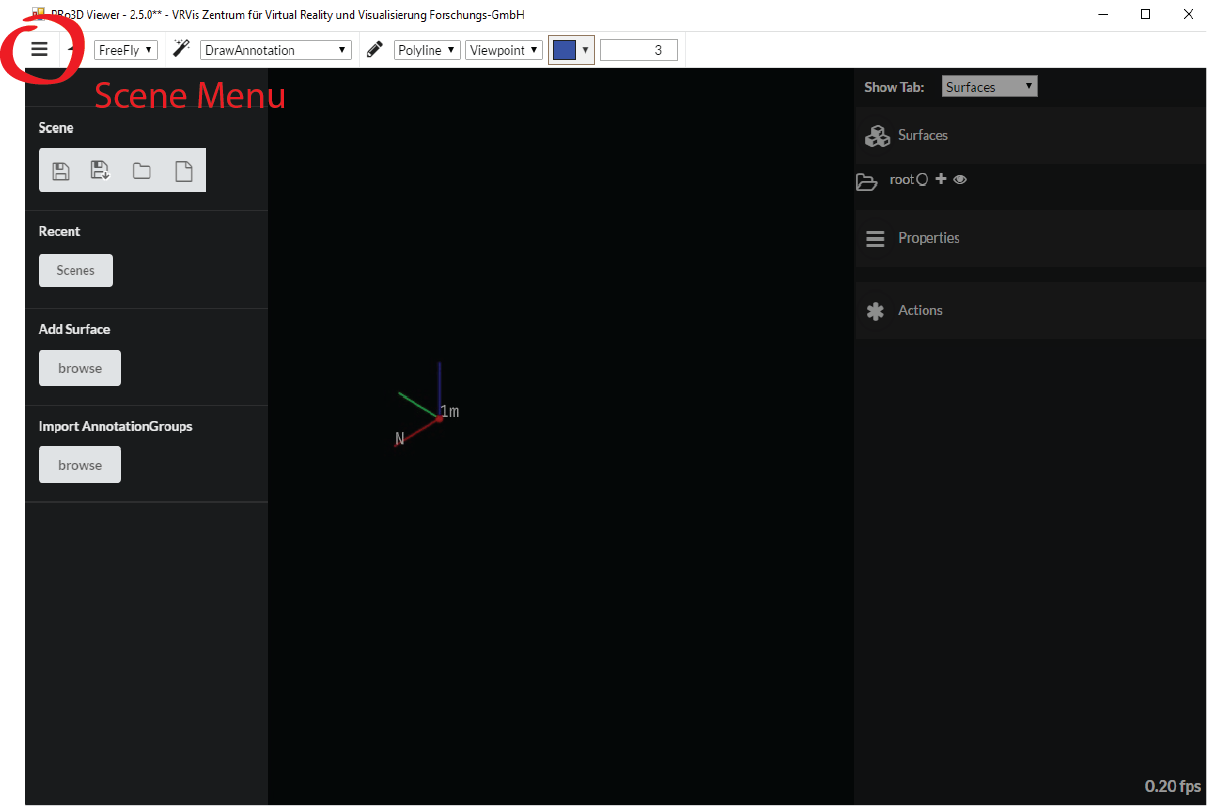
\includegraphics[width=1\textwidth]{pics/startMenuAI.png}
    	\caption[Start Menu]{Open Scene Menu. }
    	\label{fig:StartMenu}
   \end{figure}

You have two options to start:
\begin{itemize}
	\item Add one or more surfaces and create a new scene as described in the next Section~\ref{sec:addSurface}.
	\item Load an existing scene described in the Section~\ref{sec:loadScene}. 
\end{itemize}


%In the scene menu you have the following sections:
%\begin{itemize}
	%\item \textbf{Scene:}
	%\item \textbf{Recent:}
	%\item \textbf{Add Surface:}
	%\item \textbf{ImportAnnotationGroups:}
%\end{itemize}

%----------------------------------------------------------------------------------------
%	SubSection: Add Surface
%----------------------------------------------------------------------------------------
\subsection{Add Surface}
\label{sec:addSurface}

To add a new surface click the ``Browse'' button in the \textbf{AddSurface} section in the scene menu (Figure~\ref{fig:StartMenu}).
This opens the ``Select Folder'' window where you can choose the surface folder as shown in Figure~\ref{fig:AddSurface}. Click the ``Select Folder'' button to confirm your selection. The surface is loaded into the viewer and listed in the right part of the window as shown in Figure~\ref{fig:NewSurface}, part A.
You can add more surfaces in the same way.
	
	\begin{figure}[h]
    	\centering
    		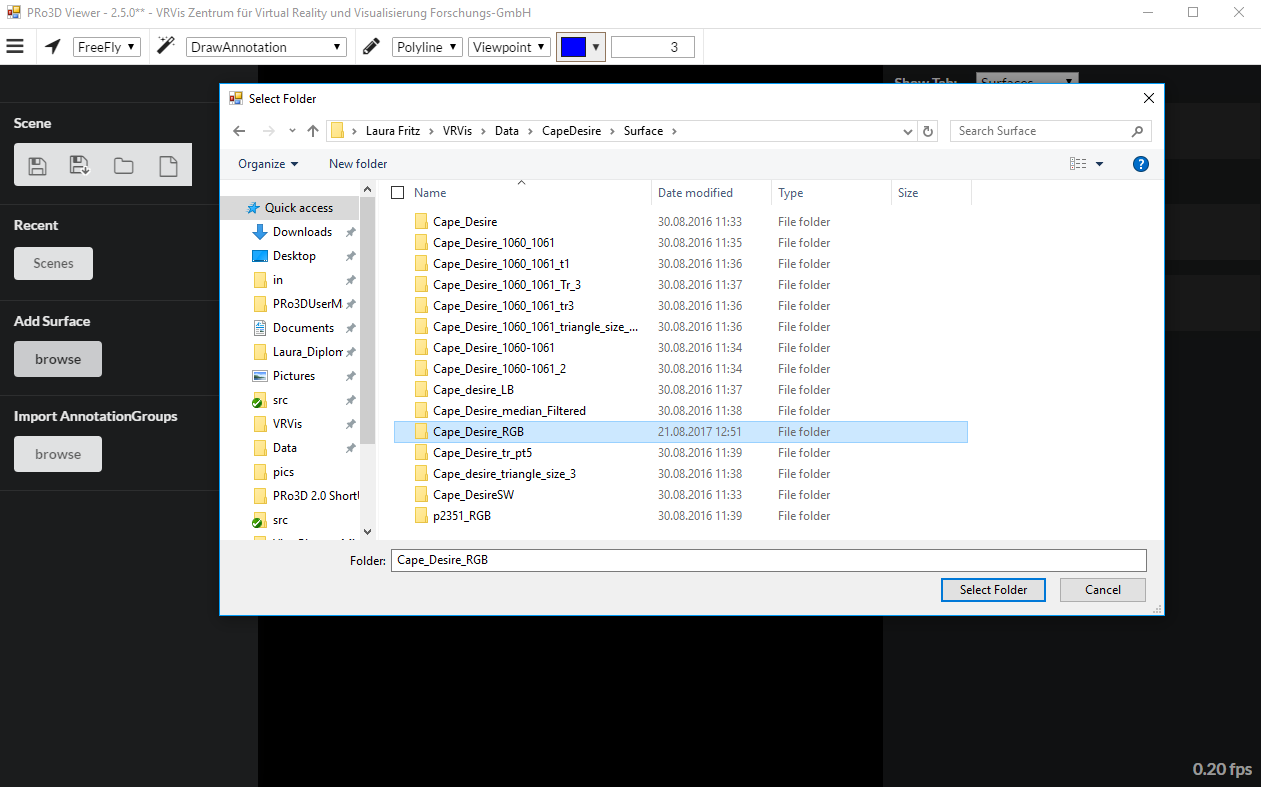
\includegraphics[width=1\textwidth]{pics/AddSurface.png}
    	\caption[Add Surface]{Add a new surface to the scene.}
    	\label{fig:AddSurface}
   \end{figure}
	
	
Each surface has a little context menu below the surface's name in the list (Figure~\ref{fig:NewSurface}, B). Click the ``FlyTo'' button to see the surface in the main window. To see the surface's properties click on the appropriate name in the list (Figure~\ref{fig:NewSurface}, C).
	
Finally, click ``SaveScene'' in the scene menu, name the scene and press the ``Save'' button (Figure~\ref{fig:saveScene}) to save the surfaces and your settings. The PRo3D viewer will load the scene automatically next time you start the viewer.
	
	\begin{figure}[h]
    	\centering
    		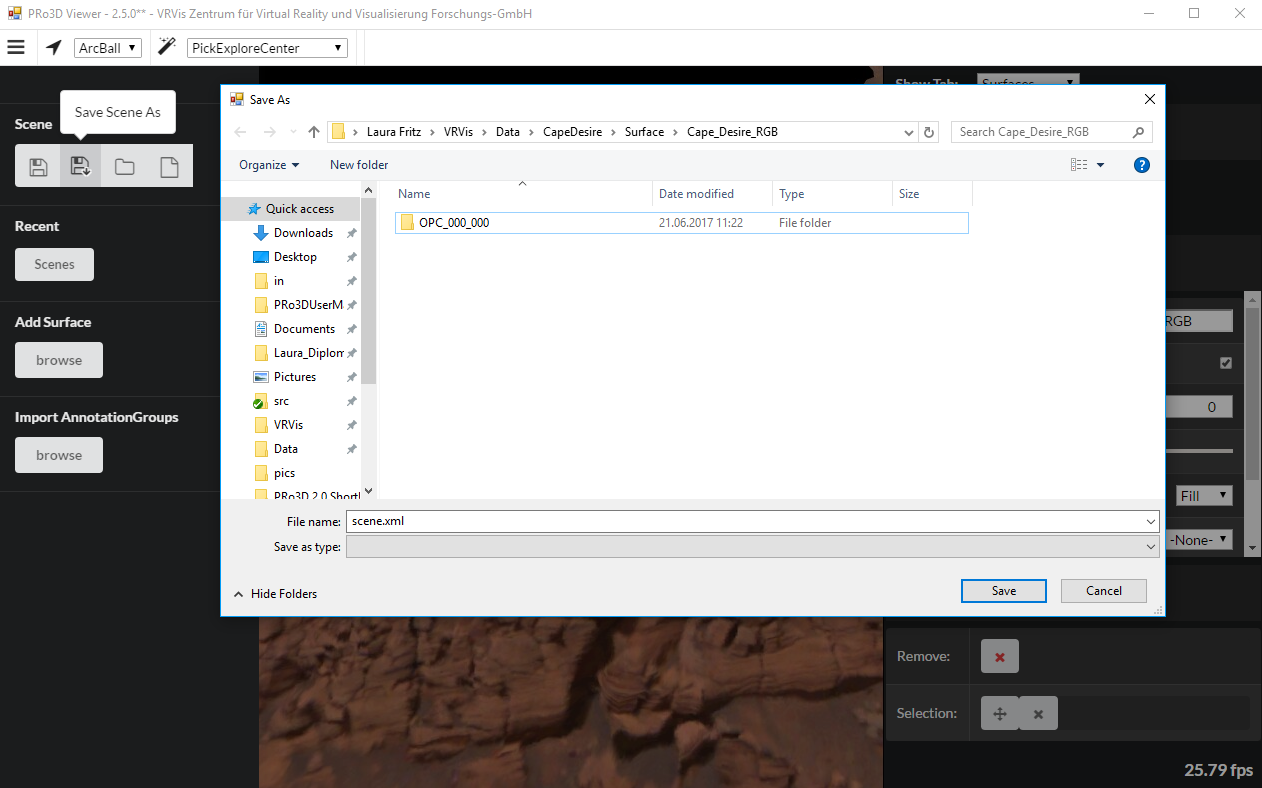
\includegraphics[width=1\textwidth]{pics/saveScene.png}
    	\caption[Save Scene]{Save the surfaces and settings as scene. }
    	\label{fig:saveScene}
   \end{figure}
		
%----------------------------------------------------------------------------------------
%	SubSection: Load Scene
%----------------------------------------------------------------------------------------
\subsection{Load Scene}
\label{sec:loadScene}

Load an existing scene by selecting ``Open Scene'' in the \textbf{Scene} section in the start menu (Figure~\ref{fig:StartMenu}).
Select the scene xml file in the directory of your choice and confirm your selection (Figure~\ref{fig:OpenScene}).
Then the scene is loaded (Figure~\ref{fig:NewSurface}). 

\begin{figure}[h]
    	\centering
    		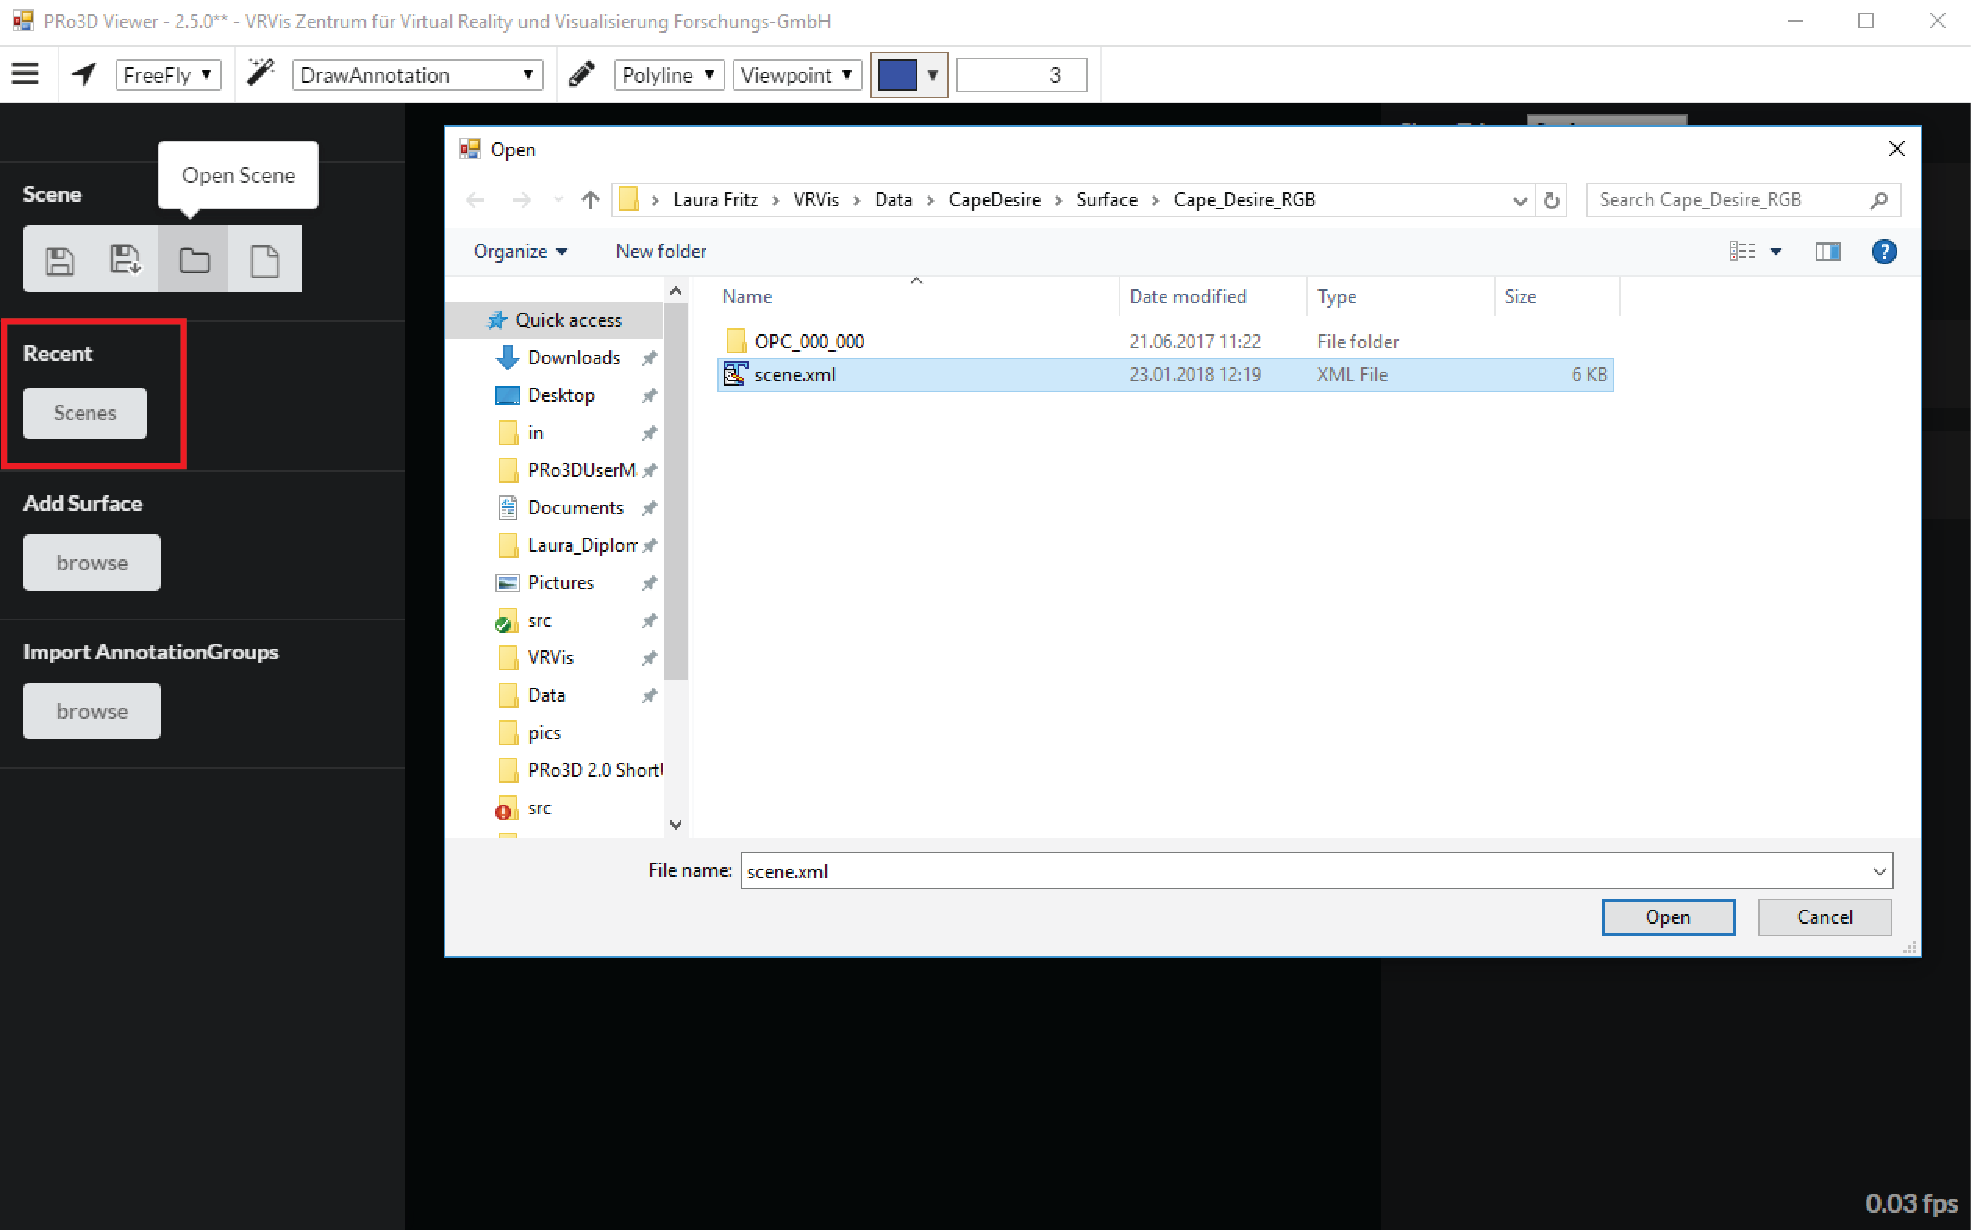
\includegraphics[width=1\textwidth]{pics/OpenSceneAI.png}
    	\caption[Open Scene]{ Open a scene with either the ``Open Scene'' button in the scene section, or with the ``Scenes'' button in the recent section (red rectangle).}
    	\label{fig:OpenScene}
   \end{figure}
	
You can also load recent scene files with the ``Scenes'' button in the \textbf{Recent} section (red rectangle in Figure~\ref{fig:OpenScene}). By hovering with the mouse over the button,
a tool tip menu with a list of recent scenes opens. Click on the required scene name to load the scene.

\begin{figure}[h]
    	\centering
    		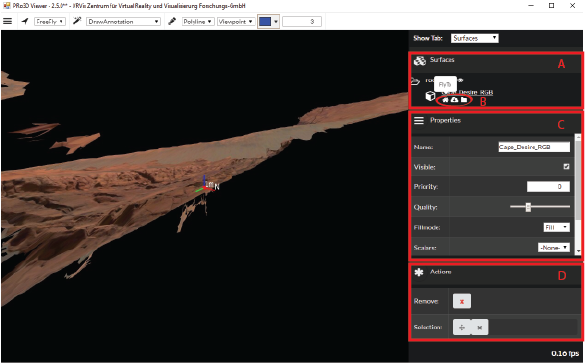
\includegraphics[width=1\textwidth]{pics/NewSurfaceAI.png}
    	\caption[New Surface]{Loaded surface with open surface features (right).}
    	\label{fig:NewSurface}
   \end{figure} 
	